\documentclass[11pt]{article} 
\usepackage{deauthor,times}
\usepackage{graphicx}
\usepackage{hyperref}
\usepackage{amsfonts,amsmath}
\usepackage{enumitem}
\usepackage{xspace} 
\usepackage{xcolor}
\usepackage{cleveref}

\newcommand{\header}[1]{\vspace{1mm}\noindent\textbf{#1}.}
\newcommand{\headerl}[1]{\vspace{1mm}\noindent\textit{#1}.}


\newcommand{\todo}[1]{\textcolor{purple}{TODO: #1.}}
\newcommand{\sg}[1]{\textcolor{blue}{STEFAN: #1.}}

\usepackage{tikz}
\newcommand*\circled[1]{\tikz[baseline=(char.base)]{\node[shape=circle,fill=black,draw,inner sep=0.6pt] (char) {\textcolor{white}{\footnotesize \textbf{#1}}};}}


\begin{document}


\title{Red Onions, Soft Cheese and Data: \\From Food Safety to Data Traceability for Responsible AI}

\author{
Stefan Grafberger, Zeyu Zhang, Sebastian Schelter\\
University of Amsterdam\\
\{s.grafberger,z.zhang2,s.schelter\}@uva.nl
\and
Ce Zhang\\
University of Chicago\\
cez@uchicago.edu}

\maketitle

\section*{Abstract}
This article presents the \method system for question answering over unstructured text, structured tables, and knowledge graphs, with unified treatment of all sources.
The system adopts a RAG-based architecture, with a pipeline of evidence retrieval followed by answer generation, with the latter powered by a 
moderate-sized
language model.
Additionally and uniquely, \method
has components for question understanding, to derive crisper input for evidence retrieval, and for re-ranking and filtering the retrieved evidence before feeding the most informative pieces into the answer generation.
Experiments with three different benchmarks demonstrate the high answering quality of our approach, being on par with or better than large GPT models, while keeping the computational cost and energy consumption orders of magnitude lower.

%!TEX root = data-validation-ml-systems.tex
\section{Introduction}
\label{sec:intro}

Machine Learning (ML) technology has become a standard component in modern software systems. Many decisions are increasingly being automated with ML and the predictions of ML models are being exposed in data products or consumed by other downstream software components. This trend gives rise to new research challenges at the intersection between Data Base Management Systems (DBMS) community and the ML community. 
%
Many of these challenges are related to data validation. In contrast to standard software systems, for which a large arsenal of testing concepts and utilities exists, testing of ML systems is difficult. Depending on the ingested data, ML systems can behave very different, and often subtle changes in the input data, that are hard to detect by humans, can lead to very different ML predictions \cite{Athalye18}. 

\newpage
This data dependency in the transformations induced by ML models is their very strength: It allows these systems to adapt to any problem setting by learning from rules defined implicitly by a data set. But this flexibility comes at a cost: The more complex and powerful ML systems become, the more difficult it becomes to validate their predictions. 

For decades ML scientists have been considering data validation rather an engineering challenge than a research problem. Recently however with more ML systems being deployed in customer facing applications newspaper headlines remind us that without proper validation of ML components we will see more racist chatbots\footnote{\scriptsize\url{https://blogs.microsoft.com/blog/2016/03/25/learning-tays-introduction/}} or fatal car crashes\footnote{\scriptsize\url{https://www.nytimes.com/2016/09/15/business/fatal-tesla-crash-in-china-involved-autopilot-government-tv-says.html}}. Scientists in the field are beginning to take this problem very seriously. There is an emergent field of research around data management tailored to ML workflows \cite{Kumar2017}. Testing, monitoring and validation of ML systems and the data ingested and produced by ML models has become a major focus of research with dedicated workshops at major conferences and a rapidly growing research community, as summarized in \autoref{sec:solutions}. Also the recent trend in ML to render models and their predictions more transparent \cite{Samek2019} can be regarded as an attempt to validate ML systems and training or prediction data \cite{Zhang2020}.
%
However to the best of our knowledge there is no commonly agreed upon data validation solution for ML systems that has reached broad adoption. Here, we argue that one of the most important factors is that {\em automating} validation of ML systems is difficult. Especially when systems learn autonomously and continuously, it can be challenging to ensure that the performance of an ML system is not shifting due to accidental or adversarial changes in the data. Given the above examples for how ML systems can fail in practice, it is obvious that ML systems require scalable, robust and automated data validation solutions. This constraint does not apply to academic research, and thus the lack of automation in ML system validation can be considered as a major blocker slowing down the transfer of the often rapidly evolving advances in ML research into robust and trustworthy customer facing products. 


\begin{figure}
\centering
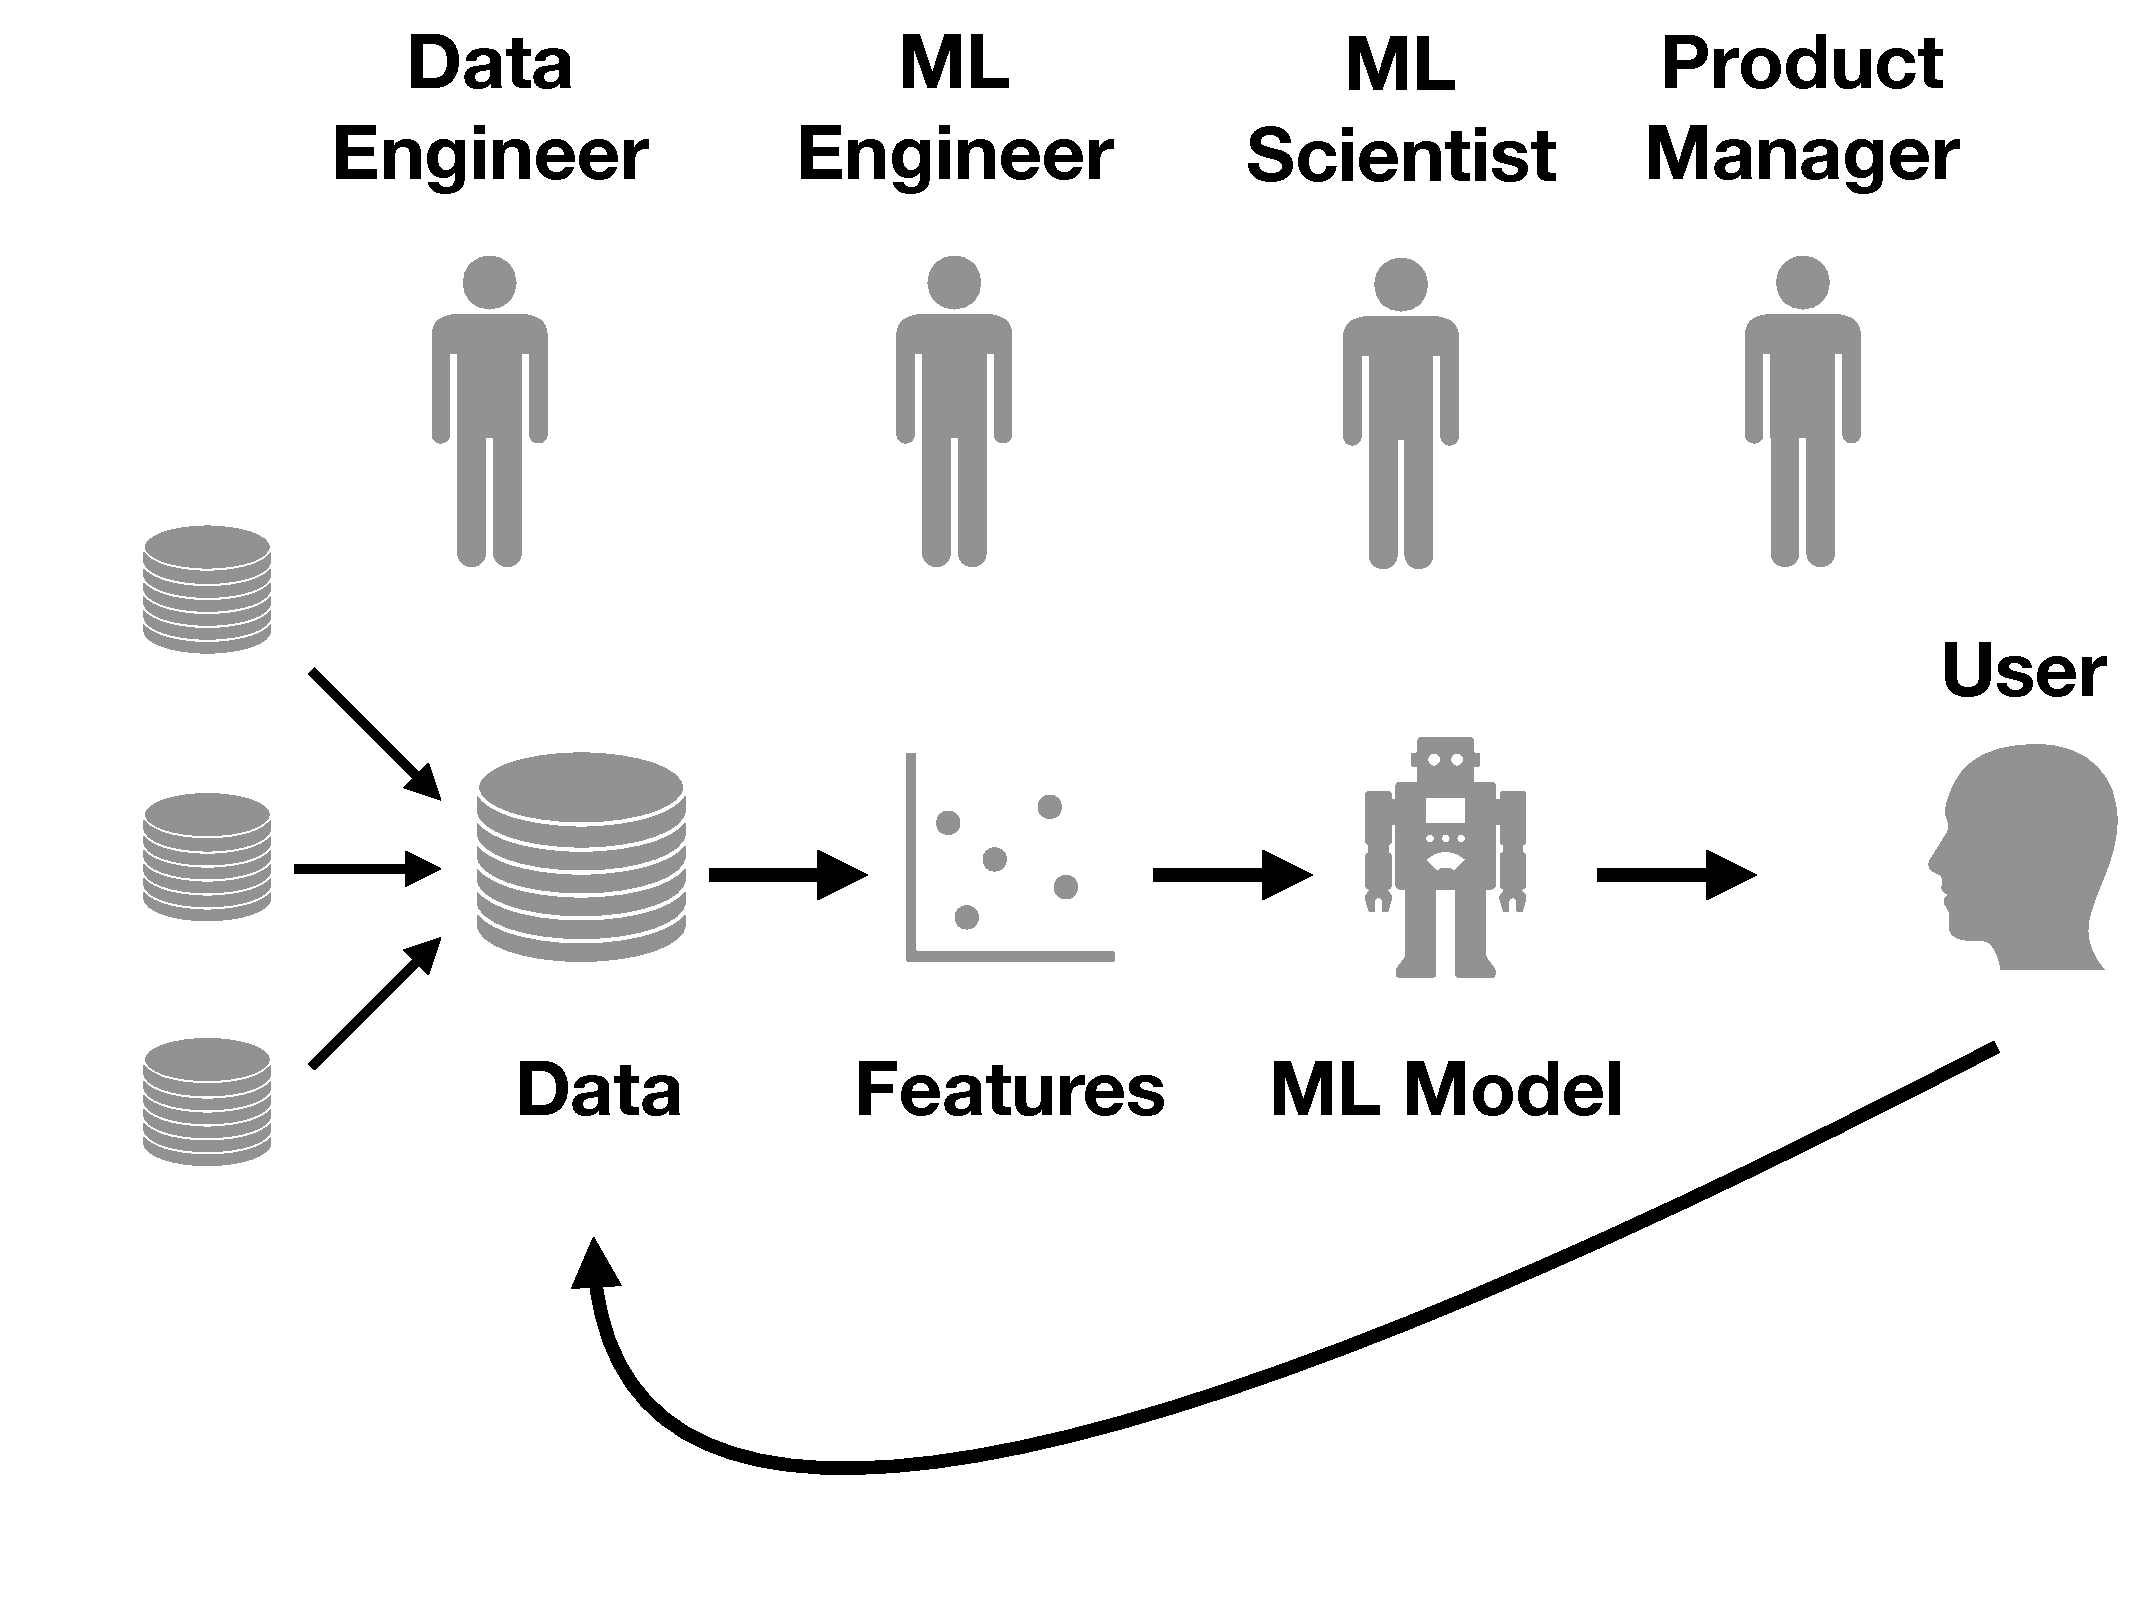
\includegraphics[width=.6\textwidth]{submissions/data-validation-amazon/figs/ML-system}
\caption{Responsibilities for a machine learning (ML) production software system are often distributed across different roles and teams \cite{Polyzotis2018}. Data from various sources is integrated, features are extracted and ML models transform these into predictions, which are then served to users whose behavioural signals are fed back to the system. Monitoring and validating these data streams at scale is only feasible with automated tests. But validating the data in each of these stages requires different competencies and often domain expertise. This imposes novel technical and conceptual challenges on engineering teams when automating ML production systems.}
\label{fig:ml-system}
\end{figure}


But why is this so difficult to automate? Researchers in the DBMS community have been investigating data profiling for decades \cite{Abedjan2018} and many of these solutions are just right for some aspects of data validation also in the context of ML systems. However some of the challenges in ML system monitoring go beyond that. Many data validation aspects in ML systems {\em depend on the state of the trained ML model}, such as the performance of a ML model under data set shift, or the differential privacy of a model \cite{Dwork08differentialprivacy, Abadi2016, Bagdasaryan2019}. Other aspects such as fairness of a ML model require domain expertise that ML engineers often do not have. As illustrated in \autoref{fig:ml-system} the competencies required to validate data in the various stages of an ML system require competencies that are usually distributed across several experts in a team or even separate teams. 

In the following chapters we will first review the challenges associated with data validation in ML systems and highlighting some of the practical implications. Afterwards we review some of the data validation solutions, with a special focus on the practical applicability of these approaches. Finally we will conclude with an outlook of technical and non-technical challenges associated with ML system validation in order to ensure more responsible usage of ML systems in production software systems. 
% !TEX root = ../main.tex
\section{What Should We Do? Food Safety as Inspiration!}
\label{sec:inspiration}

As an inspiration for the technical, data-centric vision outlined in this paper, we discuss how the US Food \& Drug Administration (FDA) combats the outbreaks of foodborne illnesses~\cite{fdaout}, and start with a concrete example.

\subsection{Example -- Outbreak of Salmonella Infections in the US in 2020} 

From June to September in 2020, a total of 1,127 people in 48 US states got infected with the outbreak strain of Salmonella Newport~\cite{fdanewport}. The FDA and the Centers for Disease Control and Prevention (CDC) managed to contain this outbreak and had the situation under control in October 2020, after which no more new infections occurred. Combatting the outbreak proceeded as follows: Sick patients from the 48 states were seeking treatment in hospitals and bacteria in their stool samples turned out to be closely related genetically, which implied a common source of infection. Subsequent epidemiologic evidence showed that over 90\% of them had eaten onions (or food made with onions) in the week before their illness. As a consequence, the FDA started a so-called ``traceback investigation'' which ultimately uncovered that red onions from the Thomson International Inc. company were the source of the Salmonella outbreak. This triggered a country-wide recall of raw onions and derived products like cheese dips, kebabs, and chicken salad sandwiches from a large number of grocery stores, which ultimately ended the outbreak.



\subsection{Disease Detectives, Traceback Investigations, and Food Supply Chains}

The remarkable success of the FDA in combatting and controlling the salmonella outbreak naturally leads to the question which processes and techniques they have applied to detect the outbreak, identify the suspect food and determine the producer of the food, and what the computer science community can learn from these battle-tested approaches.

\begin{figure}[h!]
    \centering
    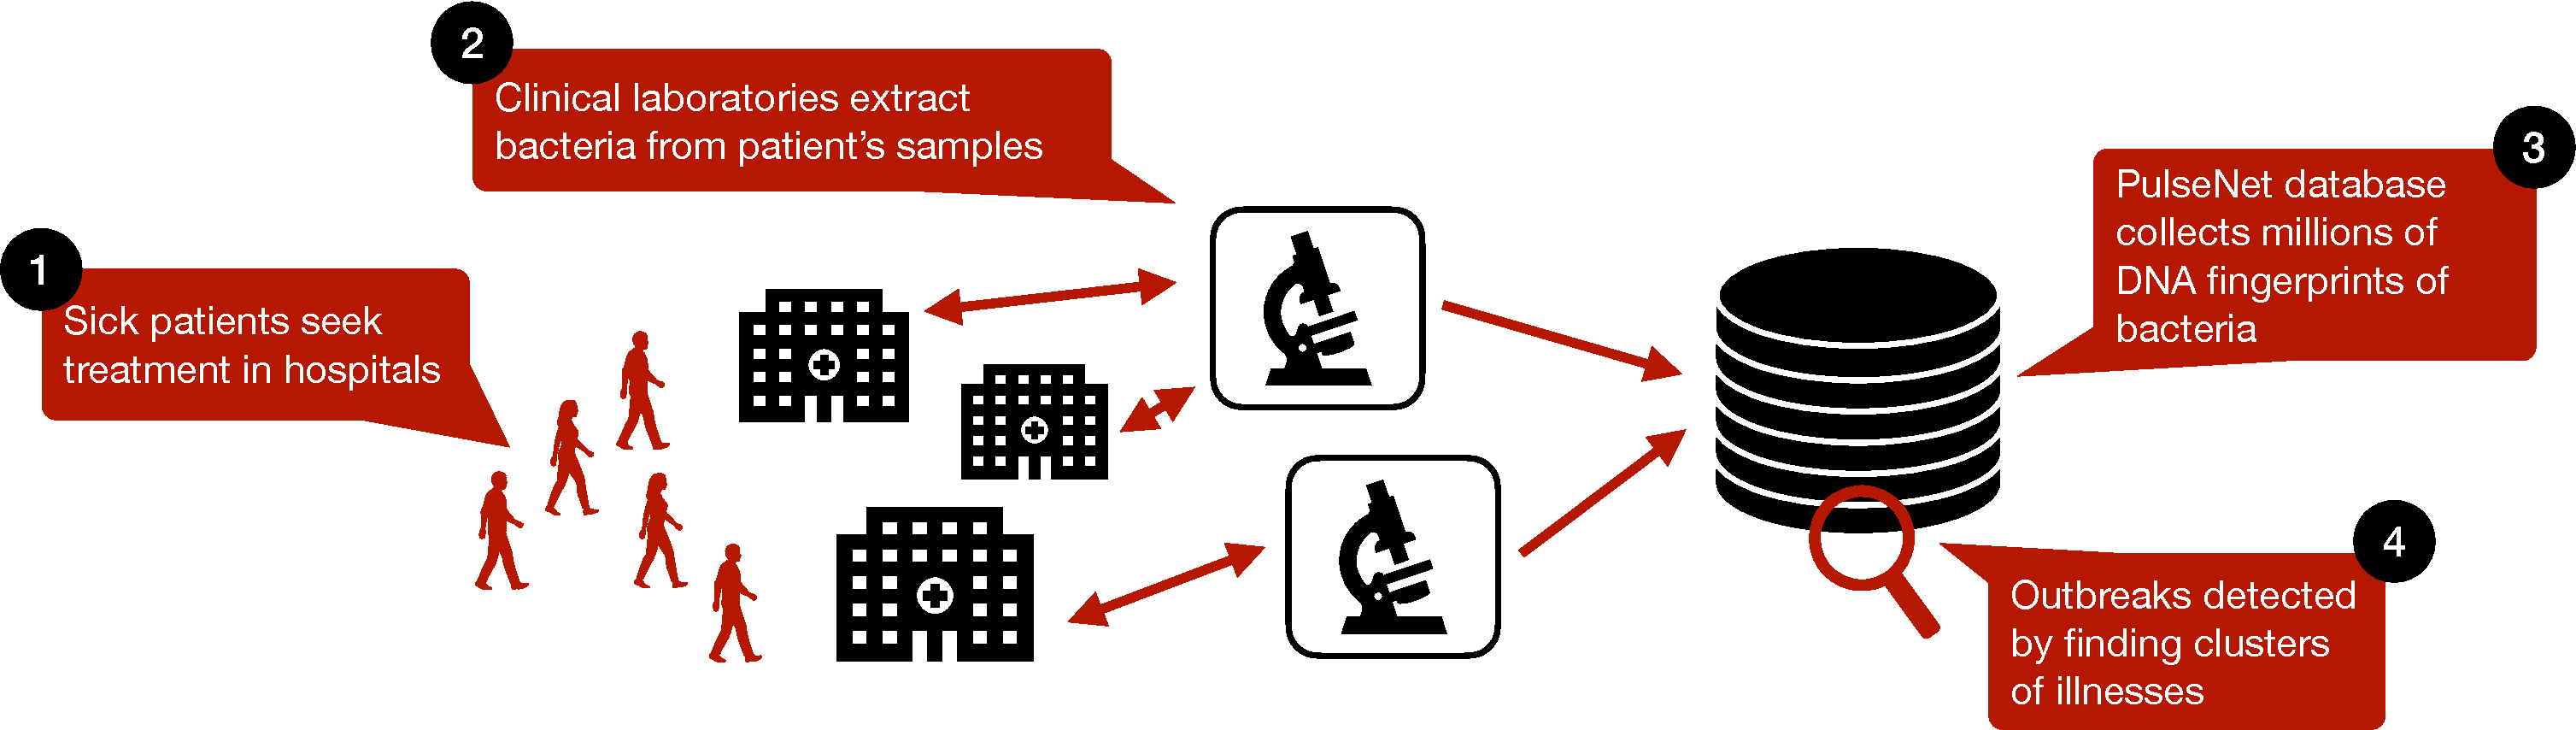
\includegraphics[width=0.8\textwidth]{submissions/submission3/figures/outbreak-detection-crop.pdf}
    \caption{Outbreak detection by monitoring a database of millions of DNA profiles of bacteria.}
    \label{fig:outbreak}
\end{figure}

\header{Outbreak detection} The first question is how the FDA actually detects that there is an outbreak of a foodborne disease. We illustrate the underlying process in \Cref{fig:outbreak}: Sick patients seek treatment in hospitals, from where their doctors send stool samples to laboratories for analysis. The laboratories perform DNA fingerprinting on the bacteria isolated from these samples via whole genome sequencing and the resulting DNA fingerprints are subsequently collected via the PulseNet system~\cite{cdcpulsenet}. PulseNet is a nationwide network of public health and food regulatory agency laboratories coordinated by the CDC and manages a national central database with millions of collected DNA profiles of bacteria. In this database, the sudden appearance of clusters of genetically related bacteria implies a common source of infection and indicates an outbreak.

\header{Identification of the suspect food} Once an outbreak is detected, the next task is to identify the contaminated ``suspect food'' which infects people. As shown in \Cref{fig:identification}, the FDA employs so-called ``disease detectives'', who contact the sick patients and interview them to gather epidemiologic evidence related to questions such as ``what foods did people eat before they got sick?'' or ``what restaurants, grocery stores, or events did sick people go to?''. For that, they leverage data provided by the patients, e.g., purchasing records collected on loyalty cards. These activities typically lead to the identification of a particular suspect food, which is likely the root cause of the outbreak.

\begin{figure}[h!]
    \centering
    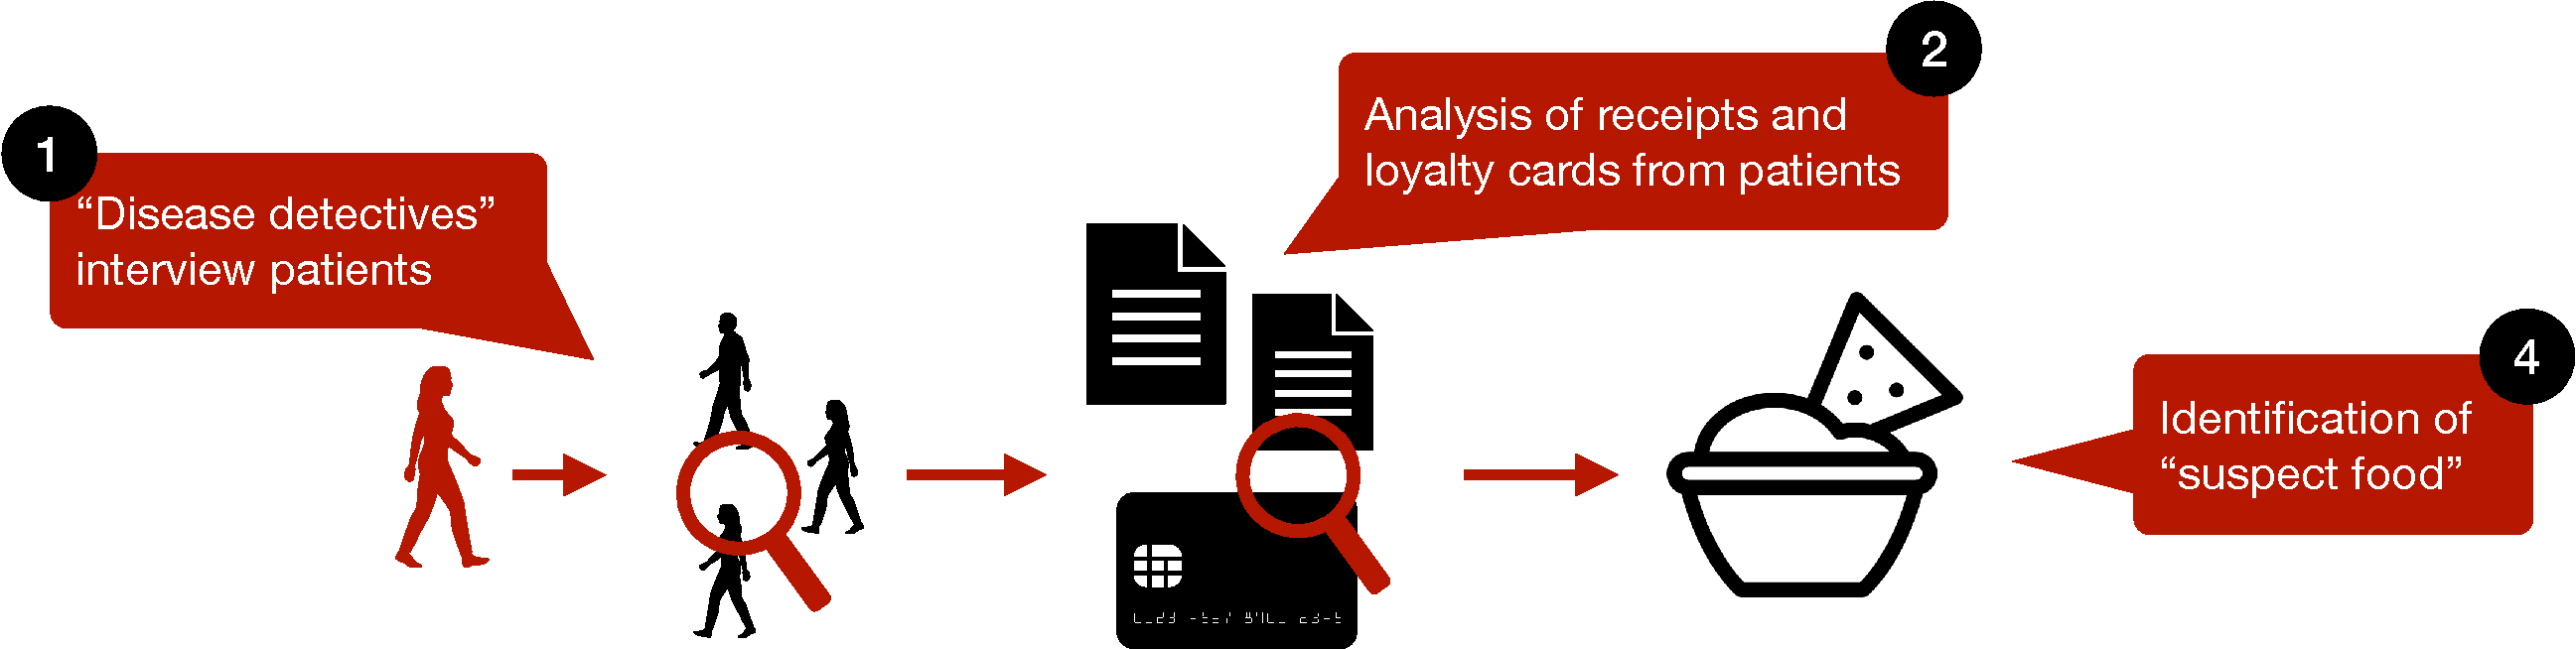
\includegraphics[width=0.8\textwidth]{submissions/submission3/figures/food-identification-crop.pdf}
    \caption{Disease detectives collect epidemiological evidence from sick patients to identify a contaminated suspect food likely causing the outbreak.}
    \label{fig:identification}
\end{figure}

\header{Traceback investigation to determine the producer of the contaminated food} Once the responsible food is known, the final task is to identify the actual point in the supply chain, where the food is likely being contaminated. For that, the FDA starts a traceback investigation through the food supply chain, as illustrated in \Cref{fig:traceback}. Here, the supply chain for several contaminated end products is traced back retrospectively to identify a common point in the supply chain which is likely the source of the contamination. 

\begin{figure}[h!]
    \centering
    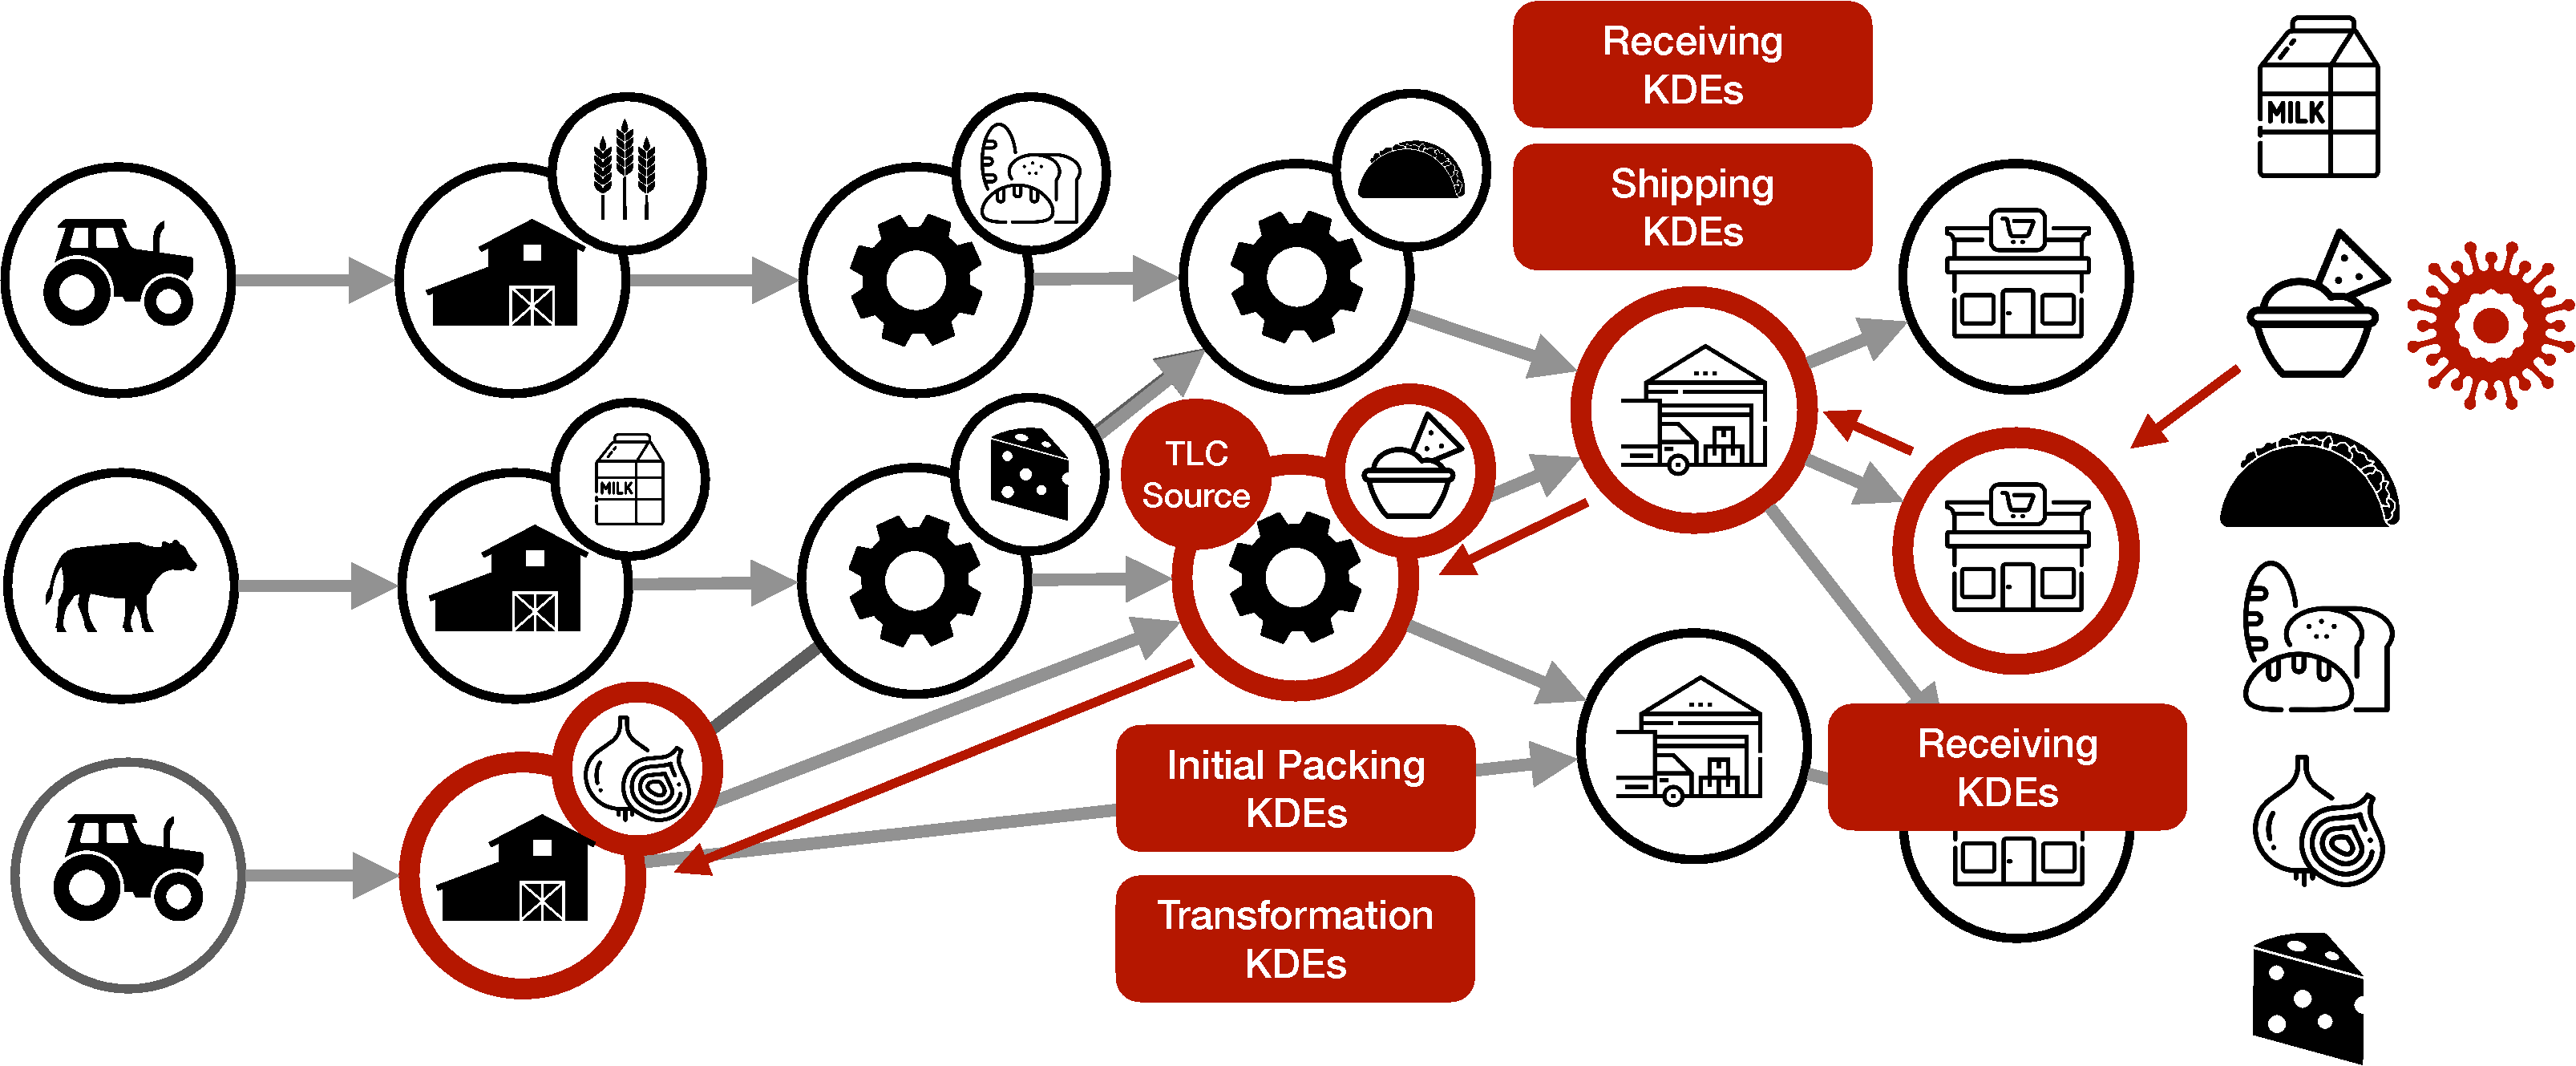
\includegraphics[width=0.8\textwidth]{submissions/submission3/figures/traceback-crop.pdf}
    \caption{Traceback investigation through the food supply chain, relying on \textit{Traceability Lot Codes} (TLCs) to identify units of food and provenance information in the form of \textit{Key Data Elements} (KDEs) to reconstruct the path a unit of food took through the chain.}
    \label{fig:traceback}
\end{figure}

For that to be possible, entities involved in the food supply chain must have followed the FDA's \textit{Food Traceability Rule}~\cite{fdafaq} and maintain traceability information for potentially dangerous food on the \textit{Food Traceability List}~\cite{fdaftl}. Such entities must maintain a \textit{Traceability Plan}, with information about procedures used to maintain traceability information and a point of contact for traceability questions~\cite{fdatp}. The food traceability rule further defines \textit{Critical Tracking Events} (CTEs) in the supply chain, where detailed tracing data must be created, maintained and forwarded by the participating entities. Examples of such events are the initial packing of a food, shipping it, or transforming multiple ingredients into a new food. An individual unit of food is assigned a \textit{Traceability Lot Code} (TLC),  typically during the initial packing event, which uniquely identifies it and is forwarded to receiving entities. Furthermore, the food traceability rule defines certain categories of \textit{Key Data Elements} (KDEs), which must be created, maintained, and forwarded together with the TLCs of the food. Examples of the different categories are \textit{Initial Packing KDEs}, \textit{Shipping KDEs}, \textit{Harvesting and Cooling KDEs} and \textit{Receiving KDEs}. The actual data items per KDE depend on the category, e.g., for the packing KDEs, the date, quantity, harvest location, name, and contact information of the harvesting company must be maintained, and the initial TLCs are typically assigned at the packing stage as well. Shipping KDEs need to include the corresponding TLCs, the shipping date, and the locations for receiving and shipping. A special case are Transformation KDEs, which must be created at points where a new food is produced from several ingredients. Here, the link to the ingredient TLCs must be recorded, as well as a location description, the transformation date, and the quantities of the ingredients.

% !TEX root = ../main.tex
\section{Towards Data Traceability for Responsible AI}
\label{sec:vision}


In this paper, we develop a technical, data-centric vision to work towards a comparable level of safety in AI/ML applications as the FDA has in combatting foodborne illnesses. Unfortunately, the current state of AI/ML safety in the industry is dire, as practitioners from the aforementioned industry survey~\cite{holstein2019improving} report that ``teams do not discover serious fairness issues until they receive customer complaints about products'' or read ``negative media coverage about their products'', and more than half of the respondents agreed that they ``discovered serious issues only after deploying a system in the real world''. While this survey paper identifies many crucial issues in this space, it unfortunately falls short of outlining concrete technical directions for addressing them. 

In the following, we outline our ideas for improving the safety of AI/ML applications. Inspired by the existing methods and processes for combatting foodborne illnesses from \Cref{sec:inspiration}, we propose ideas on ``detecting outbreaks'' via prediction monitoring in \Cref{sec:vision-monitoring}, for conducting ``traceback investigations'' through data supply chains in \Cref{sec:vision-tracing}, and for identifying ``contaminated data and pipeline steps'' through audits in \Cref{sec:vision-audit}.
% !TEX root = ../main.tex
\subsection{Prediction Monitoring}
\label{sec:vision-monitoring}

As detailed in \Cref{sec:inspiration}, the FDA monitors a database of DNA profiles of bacteria for geographic patterns to detect outbreaks. This raises the question of whether large institutions or companies could use similar methods to detect fairness issues with deployed models and ML pipelines early. In the following, we outline three directions which we deem crucial for this endeavour.

\header{Identifiable predictions} The ``end product'' of AI/ML applications are predictions on unseen data, which are received by end-users or downstream applications in an organisation. Any detection of problems with the application or its data, as well as any potential audit has to start from these predictions, similar to how disease detectives need to determine the type of food that people consumed before they became sick. However, in current systems, predictions are often rather ephemeral. As a first step towards auditable AI/ML applications, their predictions should come with unique identifiers, analogous to the TLC of food in food supply chains. Such identifiers should be assigned in a way that allows for the retrospective identification of the state of the AI/ML application (e.g., the software version and currently deployed model version, etc.) from which a prediction was generated. Based on these identifiers, users and downstream consumers could raise concerns about a particular prediction, and an investigating party (e.g., a dedicated responsible AI team in a large organisation) could start an audit of the system.

\headerl{State-of-the-art} In MLOps, the benefits of identifiable predictions are being recognised among industry practitioners~\cite{tensorflowPatterns21,howToMonitor23}. However, current approaches require high expertise and custom implementations~\cite{tensorflowPatterns21}. Even rudimentary tasks such as tracking the corresponding code and model versions are challenging~\cite{traceabilityAndReproducibility23}. To fully benefit from identifiable predictions, e.g., for rectifying erroneous predictions, it is essential to integrate prediction identifiers with the associated metadata and provenance records encompassing ancillary pipeline stages such as data preprocessing. However, the current implementation complexity leads us to believe that the adoption of these techniques in practice is rather low.
  
\headerl{Open questions and challenges} Enhancing and maintaining traceability and reproducibility in ML applications requires that practitioners manually integrate, configure, and orchestrate various disparate systems~\cite{traceabilityAndReproducibility23,tensorflowPatterns21}. The resulting one-off solutions require further time- and cost-intensive development effort to enable monitoring and output explanation. We argue that standardised interfaces would be essential to seamlessly integrate existing and new ML operations techniques with identifiable predictions.
%
We will also discuss further provenance-related challenges for fine-grained data tracing in end-to-end ML pipelines in Section~\ref{sec:vision-tracing}. 


\header{Detecting and collecting predictions with fairness issues} Even with identifiable predictions, an open question is how to reliably detect fairness issues of an ML application at deployment time. Ideally, such issues should already be caught by pre-deployment evaluations, but media reports and industry surveys show that this is rarely the case. Furthermore, it would be crucial to have a ``database'' of common issues and examples of unfair / unreliable predictions in production ML deployments, e.g., at a company-wide level. Given a comprehensive catalog of such issues and an efficient way to monitor live predictions for fairness, we could build automatable detection mechanisms similar to the outbreak detection techniques in PulseNet (\Cref{sec:inspiration}).

\headerl{State-of-the-art} A lot of recent work has focused on detecting changes in the overall distribution of the predictions or changes between the training and serving data~\cite{nigenda2022amazon}. At serving time, systems like Tensorflow Serving~\cite{olston2017tensorflow} for example employ so-called ``canary models'' to detect cases where the predictions differ between previous and newly deployed models, and several techniques analyse the distribution of the predicted labels to detect changes in the data~\cite{lipton2018detecting,schelter2020learning}. However, none of these techniques have a particular focus on determining fairness issues, which may occur in small subsets of the data only. 

Orthogonal to that, several techniques to debug prediction data offline have been developed, e.g., to detect slices of the data where a model works less well~\cite{chung2019slice,sagadeeva2021sliceline}. These approaches require simultaneous access to the model, the featurised prediction data and additional demographic side data however, which makes their application difficult in practice, especially for teams not owning the underlying AI/ML application.


\headerl{Open questions and challenges} A major difficulty in monitoring a deployed system for fairness is that the group membership information for individual predictions must be known to maintain corresponding fairness metrics. Such group membership information (e.g., about the race or gender identity of the persons involved in the predictions) is very sensitive and private information, to which a deployed serving system should ideally not even have access. Furthermore, regulation like the EU AI Act enforces strict rules for which parts of an AI/ML application such data can be used for at all. We envision that large organisation may want to create dedicated infrastructure for such cases, where predictions with identifiers from different applications are collected, the corresponding fairness metrics are maintained and SliceFinder-like algorithms~\cite{chung2019slice} are run continuously to look for subsets of the prediction data with potential issues.

A large corpus of real-world predictions from ML systems with fairness issues would also greatly enhance the ability of the academic community to work on these problems. However, it is difficult to collect such a corpus of predictions and issues due to the inherent sensitive, privacy-critical nature of the data. There are some ongoing efforts to (manually) create a comprehensive repository of ``AI incidents''~\cite{mcgregor2021preventing}, yet the underlying technical details and prediction data of the incidents are not available.


\header{Monitoring generative models for representational harms} A large part of the existing fairness literature focuses on so-called ``allocative harms'' in automated decision-making systems, which decide upon access to certain resources such as job interviews, loans or medical prioritisation~\cite{stoyanovich2022responsible,holstein2019improving}. It is difficult to choose an appropriate fairness metric for such cases, as such a choice always implies a values-based decision and trade-offs~\cite{narayanan21fairness}. On the technical side however, computing these metrics is straightforward (given access to the required data), as one essentially only has to maintain separate confusion matrices for the predictions for the groups of interest~\cite{guha2024automated}. With the rise of generative models however, we are being faced with so-called ``representational harms''~\cite{holstein2019improving}, which occur for example when generative models reproduce sexist or racist stereotypes in the images or text that they generate. 


\headerl{State-of-the-art} There is a large body of targeted studies in the NLP community, where researchers uncovered a variety of biases and stereotypes in pretrained language models. Examples include sexist stereotypes and gender bias~\cite{lucy2021gender,sheng2019woman}, anti-muslim bias \cite{abid2021persistent}, and undesirable biases towards mentions of disability~\cite{hutchinson2020social}. It is however unclear how to translate the detection capabilities of these customly designed studies into monitoring techniques for deployed real-world systems. A first interesting step in this direction is the recently proposed Spade~\cite{shankar2024spade} system, which learns assertions for safeguarding LLM outputs based on the version history of prompt edits. 

\headerl{Open questions and challenges} Due to the unpredictable nature of large generative models, generating adequate assertions or ``data unit tests'' to check for bias in their output remains a complex challenge. Having too few assertions potentially might make a system miss biased outputs, leading to unfair outcomes, while having too many assertions could slow down the system and lead to many false alarms. We expect that future approaches will generate data unit tests from predefined templates, based on manually defined assertion criteria. An orthogonal approach are so-called ``safety classifiers'' \cite{xu2021bot, dinan2022safetykit,markov2023holistic}, where a secondary model is employed to assess the outputs of a primary model for safety. Prior to the deployment phase, data will be collected where generative models are intentionally probed to induce errors, which will then be used to train a classifier to detect biased behavior.



% !TEX root = ../main.tex
\subsection{Tracing Data Through End-to-End AI/ML Applications}
\label{sec:vision-tracing}

Complex food supply chains span the globe and a single ingredient (like red onions in the example from~\Cref{sec:inspiration}) may end up in multiple end products. This makes tracing such ingredients a complicated and expensive undertaking. The FDA addresses this challenge with targeted tracing requirements which focus on only retaining tracing data for high-risk ingredients on the food traceability list (\Cref{sec:inspiration}). While tracking the provenance of data in data processing systems is a decades-old research area~\cite{tan2007provenance}, there is still little practical adoption of these techniques in real-world systems, mainly due to the incurred performance overhead of comprehensively tracking provenance through all kinds of queries, especially when they contain aggregations~\cite{amsterdamer2011provenance}.
%
Similar to the FDA's list of high-risk ingredients, the EU AI Act~\cite{euaiact} defines high-risk AI application domains, such as CV-sorting software for recruitment procedures, credit scoring denying citizens the opportunity to obtain a loan or the verification of the authenticity of travel documents. In the following, we discuss ideas for efficiently applying provenance tracking to the data pipelines in such scenarios.


\header{Selective and focused provenance tracking} As already mentioned, tracking fully fine-grained semiring provenance~\cite{green2007provenance,amsterdamer2011provenance} for every input row imposes a high performance overhead. In the food supply chain, provenance tracking focuses on predefined ``Critical Tracking Events'', which are the points in the supply chain that are crucial later for audits. We need to adopt such a methodology as well for data pipelines, which would enable us to restrict the provenance tracking efforts to data exchange and transformation operations, which actually impact the information required to audit an AI/ML application later. Furthermore, for each high-risk AI application scenario, we could define the tracking granularity, the key transformations to focus on and the information required per transformation event.  The minimum granularity of the provenance should be tailored for each use-case. For demographic data, provenance at the level of individuals might be sufficient, for facial recognition applications, more fine-grained provenance at the level of individual images may be required, however.


\headerl{State-of-the-art} In recent years, several techniques have been proposed to model ML pipeline operations and to apply database-style provenance tracking for Python code, for example via runtime instrumentation as part of mlinspect~\cite{grafberger2022data} or via static analysis as part of Vamsa~\cite{namaki2020vamsa}. These approaches have been extended in various ways, e.g., for data debugging via Shapley values~\cite{karlavs2022data} or pipeline screening during continuous integration~\cite{schelter2023proactively}. A drawback of these methods is that they rely on heuristics and well-written, declarative code to be able to infer the semantics of the pipeline operations, which leaves it unclear whether they can reliably be applied to low-quality code as well. Another family of systems, which include Amazon's ExperimentTracker~\cite{Schelter2017} and mltrace~\cite{shankar2022observability}, uses a more robust approach for provenance tracking as they require manually annotated code. Unfortunately, this puts a heavy burden on developers, who will, in our experience, often forego the additional effort of putting detailed annotations on their code under time pressure. We expect that even coming up with high-level ``traceability plans'' for large AI/ML applications will be challenging in practice, since these applications often orchestrate different systems and libraries with workflow managers like Apache Airflow~\cite{airflow}.

\headerl{Open questions and challenges} In our eyes, the biggest challenge in this space is to find ways to reduce the implementation-, annotation-, and runtime overhead for provenance tracking in ML pipelines, while guaranteeing a high level of correctness and robustness. For industry applications, we can neither rely on trying to handle arbitrary code nor on forcing developers to always manually annotate their code. An interesting middle ground may be the use of pipeline templates, as pioneered by the mlflow recipes project~\cite{zaharia2018accelerating}, which forces developers to modularise their code into pipeline steps with known semantics and predefined inputs and outputs, but still gives them the freedom to write arbitrary code inside the steps. Unfortunately though, the real-world adoption of these templating approaches is unclear at the moment. Nevertheless, such templates might be a natural point to implement general robust provenance tracking. Analogous to the traceability plans required for food chain tracking, we could define traceability templates for high-risk AI scenarios, with steps, provenance tracking, and logging requirements specific to the particular use case. 

To reduce the runtime overhead of provenance tracking, it may be worthwhile to take a deeper look at several common aggregation operations in ML pipelines, like one-hot-encoding a particular column or normalising a feature. While these operations technically conduct a global aggregation followed by a map transformation (in dataflow terms), we may be able to ignore the aggregation part for tracking provenance, as we already know that they do not remove rows and introduce an all-to-all provenance relationship onto the transformed feature values. Similar techniques are already applied in DataScope~\cite{karlavs2022data} and ArgusEyes~\cite{schelter2023proactively} to approximate ML pipelines as queries in the positive relational algebra. A future challenge here is to define a restricted subset of operations for ML pipelines, which still allows the implementation of a large class of ML applications, but drastically simplifies provenance tracking.


Identifiable predictions, as discussed in Section~\ref{sec:vision-monitoring}, also present new challenges with respect to ML provenance research. Existing experiment tracking tools like mlflow~\cite{zaharia2018accelerating} already link predictions to high-level artifacts such as models and source code. However, we think that record-level provenance is required to effectively reconstruct the necessary data for a prediction. Given a prediction identifier, we would like to be able to automatically retrieve all relevant inference inputs, data preprocessing steps, the model version employed for inference, and, if necessary, all information about the training pipeline and its input data. While existing research partially addresses provenance tracking and versioning in static pipelines with static input data, further challenges remain for pipelines in dynamic production environments with continuously trained models~\cite{baylor19tfxContinous} and evolving retrieval corpora~\cite{Guo16traditionalIR,chend23dynamicCorpora,bleifuss2018change}, where provenance has to be maintained incrementally.


Another open question is the impact of data cleaning and integration operations on the fairness of AI/ML applications. Several experimental studies indicate that data wrangling and integration operations such as missing value imputation, outlier removal, or entity matching can sometimes negatively impact the fairness of models trained on the resulting data~\cite{guha2023automated,li2021cleanml,tae2019data,shahbazi2023through}. However, we currently lack a detailed understanding of this impact, especially since the outcome seems to heavily depend on the chosen fairness metric and group definition. Furthermore, determining such impact is hard in practice without access to the downstream models.

An orthogonal challenge in this area is the tension between detailed provenance tracking and the protection of private user data. Provenance tracking requires storing information about the intermediate outputs of pipeline operations and must additionally maintain sensitive metadata such as demographic group memberships of certain records to be able to quantify the fairness impact of different operations. In many cases, such sensitive metadata may not be accessible in inference systems at prediction time, for example, and measures must be taken to ensure that these sensitive attributes are only used for testing models but not for training them~\cite{euaiact}. To the best of our knowledge, current ML platforms lack support for such use cases.


\header{Provenance of data in pretrained and fine-tuned models} Academic ``textbook'' ML commonly assumes that a single dataset is used to create a particular ML model, which implies that we would only need to track the provenance of this source data through the corresponding ML pipeline. However, this assumption has never held up for real-world deployments, which typically leverage a variety of data sources as input for a pipeline and often apply ML already as part of the preprocessing of this data. Twitter's recommender system for example aggregates multiple input networks (representing likes, follows etc on the platform) into a common network dataset called RealGraph~\cite{kamath2014realgraph}, via a dedicated classifier that estimates the interaction probability between different users of the network. Several recommendation algorithms consume this aggregated dataset instead of the raw input datasets and the provenance of an interaction such as a like or follow is unclear after the transformation. This problem is exacerbated nowadays due to the prevalence of large pretrained models, which are downloaded from repositories such as HuggingFace and tailored to a particular ML use case via fine-tuning. In the majority of cases, the connection to the underlying training data becomes unclear after fine-tuning, as the current infrastructure does not keep track of the relationships between models. It would, for example, be difficult to identify all computer vision models that originate from the recently retracted LAION dataset. The situation is even worse for non-open source models created by commercial companies, where the underlying training data is not known for the base model already.

\headerl{State-of-the-art} Common methods to voluntarily document the origin of data and ML models are datasheets~\cite{gebru2021datasheets} and model cards~\cite{mitchell2019model}. These are a form of manually created, semi-structured documentation, which is, for example, in use at the popular model and data repository HuggingFace.
%
Tensorflow ML Metadata~\cite{Katsiapis2020tfx} is a library for recording and retrieving metadata associated with ML workflows. The Model Card Toolkit~\cite{fang2020introducing} supports the creation of Model Cards and can also use metadata from ML Metadata to prepopulate information such as class distributions and performance metrics. DAG Cards~\cite{tagliabue2021dag}, inspired by model cards, have also been proposed as a form of documentation, which can be automatically generated from ML pipeline code~\cite{berg2019open}. Experiment tracking tools like mlflow~\cite{zaharia2018accelerating} can log metadata as a starting point for creating documentation for ML models. OpenML~\cite{rijn2013openml} is a popular platform for sharing datasets, ML tasks, workflows, and experimentation runs. While it supports documentation like a dataset description for dataset uploads~\cite{OpenMLDatasetUpload}, it does not enforce their quality and prioritises a frictionless user experience over documentation completeness. However, OpenML automatically analyses uploaded datasets to compute additional data quality statistics. For ML pipelines, it relies on extensions for popular libraries like scikit-learn that can automatically create a serialisable description~\cite{OpenMLDocs}. Systems like Macaroni~\cite{li2023macaroni} allow querying the existing metadata in open repositories, based on a unified representation~\cite{li2023metadata}.

\headerl{Open questions and challenges} The main drawback of model cards and datasheets is that creating and maintaining helpful documentation still mostly depends on the goodwill of the parties involved in the creation of the models and the data. Most importantly, this documentation is not machine-readable in a way that would make it easy to audit and/or verify the claims made about the provided models and data. As discussed, models are nowadays often downloaded and fine-tuned programmatically (e.g., via the popular transformers library from HuggingFace~\cite{huggingtransformers}). Such packages and the underlying infrastructure pose a direct opportunity to automate provenance tracking and to record the relationships between models. The semi-automated metadata collection tools can export implementation details for reproducing experiments, however, they still put the burden to extract information about the ML pipelines and models onto the users. Recently proposed approaches such as mlwhatif~\cite{grafberger2023mlwhatif} might be a starting point to automatically extract meaningful metadata, e.g., for nutritional labels in ranking~\cite{yang2018nutritional,stoyanovich2019nutritional}.


Another recent trend are parameter-efficient fine-tuning methods~\cite{hu2021lora,li2021prefix,liu2023gpt,lester2021power}, which do not create a full model copy, but only learn a continuous prompt or an ``adapter'' to the model. In such cases, we would need to track provenance on the level of these prompts and adapters (which might later even be further combined~\cite{shah2023ziplora}). A final challenge with tracking the provenance of data in generative models is that many large datasets commonly used for these models (e.g., LAION~\cite{schuhmann2022laion} or gitschemas~\cite{dohmen2022gitschemas}) for generative models consist of links to resources on the web, which are often crawled and filtered to build a custom dataset. This filtering process must also be taken into account for provenance.



% !TEX root = ../main.tex
\subsection{Identifying ``Contaminated'' Data and Pipeline Steps Through Audits}
\label{sec:vision-audit}

It is still unclear how to efficiently and comprehensively audit AI/ML applications; see~\cite {birhane2024ai,sandvig2014auditing} for a discussion on the current state of this endeavor. Due to our data-centric perspective, we focus on issues and directions for quantitative data audits only.
%
As discussed in \Cref{sec:inspiration}, traceback investigations in the food supply chain allow disease detectives to audit these supply chains, identify the point of contamination, and ultimately remove the source of contamination by issuing comprehensive recalls for all affected end products. How can we audit AI/ML applications in a similar manner, based on the provenance information from \Cref{sec:vision-tracing}? Ideally, we would like to be able to quickly identify ``contaminated'' data and intermediate outputs, which, for example, contain unwanted stereotypes or has been rendered unrepresentative due to biased filtering operations. Once such contaminated data is identified, an audit would furthermore need to determine which models and predictions were affected and need to be retracted and/or recomputed. Furthermore, such data-centric audits should be able to answer a larger set of related questions about the robustness and regulatory compliance of an AI/ML application. Examples of such questions are what data and features were used by the application and whether this usage was in line with legal requirements (e.g., from the EU AI Act~\cite{euaiact}), or whether the application follows the timely data deletion requirements imposed by the right to be forgotten from GDPR~\cite{GDPRart17}. Furthermore, audits should be able to assess whether an application is robust enough against potential errors and changes in the data, and whether appropriate measures have been taken to quantify and control the fairness of its predictions. 


\headerl{State-of-the-art} The validation of ML data in popular ML platforms such as Google TFX~\cite{baylor2017tfx} or Amazon SageMaker~\cite{nigenda2022amazon} relies on libraries such as Tensorflow Data Validation (TFDV)~\cite{breck2019data} and Deequ~\cite{schelter2018automating,schelter2019differential}, which generate validation rules based on heuristics and data profiling. Related approaches are to ``lint'' ML data based on well-known practical issues~\cite{hynes2017data}. Follow-up work to these approaches~\cite{redyuk2021automating,shankar2023automatic} applies a technique called ``partition summarisation'' to learn to spot data with potential quality issues by applying anomaly detection based on the statistics of previously observed data partitions.

There has been extensive research on cleaning datasets, e.g., ~\cite{Ziawasch2016errors,mahdavi2019raha,jager2021benchmark,narayan2022can}. Furthermore, the data-centric AI community started developing related techniques that jointly consider the ML model and data to address inaccuracy, bias, and fragility in real-world ML applications and are tackling tasks such as training set selection and data acquisition~\cite{mazumder2023dataperf}. Many of the techniques in this space rely on data influence estimation techniques~\cite{hammoudeh2022training}, in particular on (an estimate of) the leave-one-out error or data Shapley value~\cite{ghorbani2019data}, which is either computed via extensive retraining or influence functions~\cite{pmlr-v70-koh17a}. Such techniques are the basis of several recently proposed data debugging methods like Rain~\cite{wu2020complaint}, Gopher~\cite{pradhan2022interpretable} or DataScope~\cite{karlavs2022data}. 
%
A related line of work tackles ML pipelines and employs light-weight provenance tracking and automatic instrumentation of Python code to assess technical bias introduced by sudden distribution shifts~\cite{grafberger2022data,grafberger2021demo}, data leakage and fairness issues~\cite{schelter2022screening,schelter2023proactively}, as well as robustness to erroneous input data~\cite{grafberger2023mlwhatif,grafberger2023demo}. 


\headerl{Open questions and challenges} 
Unfortunately, neither TFDV nor Deequ have a particular focus on identifying fairness and bias issues in the data, and require a relatively high user expertise and knowledge of the underlying domain to adjust and filter the suggested validation rules. It would be crucial to find ways to guide users in designing compliance- and fairness-related data unit tests with these libraries. 

Furthermore, the existing methods for estimating the influence of training samples are extremely restricted in terms of efficiency, scalability or applicability. In general, there exist two families of methods: Retraining-based methods are applicable to any model class, but require extensive retraining of the ML model on a large number of subsets of the data. Even retraining a model a few hundred times for a large dataset is infeasible in practice. The second family are gradient-based methods, which require no retraining but are only applicable to certain model classes due to assumptions of convexity~\cite{pmlr-v70-koh17a} or linearity~\cite{yeh2018representer}, and are still rather compute-heavy, as they often require to compute a ``Hessian vector product'' for each combination of a training and validation sample~\cite{hammoudeh2022training}. Some exciting progress has been made in terms of scalability, e.g., on efficiently computing the Data Shapley value~\cite{ghorbani2019data} for kNN proxy models~\cite{jia2019towards}. However, these techniques are only applicable to certain utility functions but, for example, not to common ranking-based metrics in information retrieval.

The work from the data-centric AI community is promising. However, challenges such as ML pipelines with complex data preprocessing operations are often overlooked, and automatically applying these techniques to ML pipelines is still an open challenge~\cite{grafberger2023towards}. The approaches for the holistic screening of ML training pipelines rely on well-written code, which is often an unrealistic assumption in practice. 

On the engineering side, we should strive to design a standardised API for provenance-based data auditing and incident investigation, which could be integrated into popular projects such as Google TFX, mlflow recipes, or SageMaker. Based on such an API, the academic and open source community could develop general auditing software to greatly reduce the costs of such audits.

%!TEX root = data-validation-ml-systems.tex
\section{Conclusion}
\label{sec:conclusion}

Validation of input and output data in ML production systems has many facets that require competencies often distributed across a heterogeneous team of engineers and scientists, as illustrated in \autoref{fig:ml-system}. While some of the data validation challenges, such as schema validation or data consistency, can be tackled with traditional data profiling methods established the DBMS community, other validation dimensions are specific to ML systems. These ML model dependent validation challenges include aspects like accuracy and robustness under data shifts, fairness of ML model predictions and privacy concerns. 

In \autoref{sec:solutions} we highlight a number of solutions to validate single aspects. Many of these approaches are typically tailored to specific use cases and often require considerable integration efforts in production ML systems. 
A good example are the various solutions from both the ML community as well as the DMBS community for checking simple data properties, such as the data types, and also more complex dimensions like data consistency. Many of these approached allow for automating the generation of validation checks. Yet in practice it is not trivial to automate the generation of validations for a new ML system that ingests and produces millions of rows and columns. For instance, there are many cases when simple validation checks on input data will lead to false alarms when shifts or errors in a single feature do not impact the output of a downstream ML model -- maybe because that feature was neglected by the ML model, when strong regularization during the ML model training phase taught the model to ignore that feature. 

Despite the rapid progress in recent years to automate and monitor ML systems: to the best of our knowledge there exists no data validation system that has reached broad adoption and which takes into account all of the data validation dimensions sketched in \autoref{sec:dimensions}. One reason for this is the difficulty of combining the multitude of validation strategies listed in \autoref{sec:solutions} into one unified framework. Considering the rapid pace of research at the intersection of ML and DBMS, see for instance \cite{Dong2018}, it is fair to assume that it is merely a matter of a few years until one framework or some open standard for data validation in the context of ML systems will have reached broad adoption. 

There are many data validation challenges in ML systems that go beyond technical aspects. Many of them are due to the complex nature of the data transformations induced by ML models. For instance identifying unfair biases often requires domain knowledge or access to grouping variables, which are often not available. And even if those are available, it is not always clear how fairness in the context of ML systems can be defined  \cite{Zhang2020}. A conceptual challenge related to privacy is for instance the trade-off between utility and differential privacy of a ML system \cite{Jayaraman2019}: how much predictive accuracy should be sacrificed to ensure privacy? Sacrificing accuracy against privacy in domains like health care or jurisdiction is a difficult question for which ethical and legal dimensions are more important than technical aspects. Next to these ethical and legal aspects, there is one key factor hindering adoption of comprehensive data validation in ML systems and that more related to cultural aspects. Many scientists like to build new models and tools, but writing tests, integrating monitoring and validation stages in an ML system are not exactly the most popular tasks amongst researchers. But often the competencies of the scientists who built a model is required to build well functioning monitoring and validation solutions in ML systems. 

Based on these observations we derive some suggestions for how to drive innovation and adoption of data validation in the context of ML systems. First, we hope that the current trend for research at the intersection of ML and DBMS communities will continue to grow and identify more synergies leveraging and complementing each others expertise. We have seen some great examples of constructive but vivid discussion between the two communities, for instance that sparked by Kraska and colleagues around their work on learning index structures \cite{Kraska2018}. This work is unrelated to data validation and mentioned merely as an example of transdisciplinary research debates. 
Second, when building ML systems there is a broad spectrum of operational challenges and seamless integration with cloud infrastructure is key to reaching broad adoption. 

\newpage
We conclude that establishing data validation in ML systems will require a stronger focus on usability and simple APIs. Third we believe that data validation in ML systems will reach broad adoption once the research community will have found better ways of automating the validation workflow, most importantly the generation of checks for each of the data validation dimensions listed in \autoref{sec:dimensions}. 

In the past years we have seen great examples of automated tooling for tracking ML experiments \cite{Schelter2017}, experimentation in ML production systems \cite{Bose2017a}, input data validation \cite{Schelter2018,Breck2019} and validation strategies for predictions of ML systems \cite{Rabanser2018,Schelter2020,DAmour2020}. One example of how some of these data validation techniques could be integrated into an automated workflow would be that presented in \cite{Rukat2020}, where the authors propose to iterate through a sequence of data validation~\cite{Schelter2018}, data cleaning\cite{Biessmann2018a} and quantification of downstream impact on ML predictive performance~\cite{Schelter2020} to achieve an automated ML workflow. We believe that increasing the level of usability through automation in data validation will enable researchers to focus on more important questions like the conceptual, ethical and legal questions and ultimately lead to more responsible usage of ML systems in production systems.

\newpage
\bibliographystyle{plain}
\bibliography{submissions/submission3/main}
\end{document}
